\documentclass{ltjsarticle}

% packages
\usepackage{listings}
\usepackage{graphicx}
\usepackage{amsmath}
\usepackage{color}
\usepackage{here}

% document data
\title{プログラミング系レポートテンプレート}
\date{} % 日付を出力しない
\author{toma09to}

% base16-default-light
\definecolor{base00}{rgb}{0.96875,0.96875,0.96875}
\definecolor{base01}{rgb}{0.90625,0.90625,0.90625}
\definecolor{base02}{rgb}{0.84375,0.84375,0.84375}
\definecolor{base03}{rgb}{0.71875,0.71875,0.71875}
\definecolor{base04}{rgb}{0.34375,0.34375,0.34375}
\definecolor{base05}{rgb}{0.21875,0.21875,0.21875}
\definecolor{base06}{rgb}{0.15625,0.15625,0.15625}
\definecolor{base07}{rgb}{0.09375,0.09375,0.09375}
\definecolor{base08}{rgb}{0.66796875,0.2734375,0.2578125}
\definecolor{base09}{rgb}{0.859375,0.5859375,0.3359375}
\definecolor{base0A}{rgb}{0.96484375,0.7890625,0.53125}
\definecolor{base0B}{rgb}{0.62890625,0.70703125,0.421875}
\definecolor{base0C}{rgb}{0.5234375,0.75390625,0.72265625}
\definecolor{base0D}{rgb}{0.484375,0.68359375,0.7578125}
\definecolor{base0E}{rgb}{0.7265625,0.54296875,0.68359375}
\definecolor{base0F}{rgb}{0.62890625,0.41015625,0.2734375}

% listings C definition
\lstdefinelanguage{myC}{
    % Keywords
    morekeywords=[1]{auto,break,case,char,const,continue,default,do,double,else,enum,extern,float,for,goto,if,int,long,register,restrict,return,short,signed,sizeof,static,struct,switch,typedef,union,unsigned,void,volatile,while,\_Bool,\_Complex,\_Imaginary},
    % Values
    morekeywords=[2]{true,false,NULL,-20,-19,-18,-17,-16,-15,-14,-13,-12,-11,-10,-9,-8,-7,-6,-5,-4,-3,-2,-1,0,1,2,3,4,5,6,7,8,9,10,11,12,13,14,15,16,17,18,19,20}, % 自動化できないことはないが面倒くさい
    moredelim=[l][\color{base0C}]{\#}, % Preprocessor
    morecomment=[l]{//},
    morecomment=[s]{/*}{*/},
    morestring=[b]{\"},
    morestring=[d]{\'},
    alsoletter={-1234567890},
    frame=none,
    breakatwhitespace=false,
    breaklines=true,
    captionpos=t,
    keepspaces=true,
    numbers=left,
    numbersep=5pt,
    showspaces=false,
    showstringspaces=false,
    showtabs=false,
    tabsize=4,
    backgroundcolor={\color{base00}},
    basicstyle={\small\ttfamily\color{base05}},
    commentstyle={\small\ttfamily\color{base03}},
    keywordstyle=[1]{\small\ttfamily\color{base0E}},
    keywordstyle=[2]{\small\ttfamily\color{base09}},
    stringstyle={\small\ttfamily\color{base0B}},
}

\begin{document}
\maketitle
\section{ソースコードと段落}
これは本文です。このようにある程度長い文章を書いてみると、きちんと段落の先頭で字下げが行われていることがわかります。
\TeX ファイル内で改行しても、そのまま前の文章につながって出力されます。 \\
強制的に改行したいときは末尾に\textbackslash\textbackslash を入れます。

空行を挟むと段落が変わります。
\subsection{ソースコード}
以下がソースコードの例です。
\begin{lstlisting}[language=myC,caption=FizzBuzz問題の1つの解法]
#include <stdio.h>
#define NUM 20

int main(void) {
    for (int i = 0; i < NUM; i++) {
        if (i % 15 == 0) {
            printf("FizzBuzz\n");
        } else if (i % 3 == 0) {
            printf("Fizz\n");
        } else if (i % 5 == 0) {
            printf("Buzz\n");
        } else {
            printf("%d\n", i);
        }
    }

    return 0;
}
\end{lstlisting}

\section{図表の挿入}
以下のように図や表を挿入することが出来ます。
\begin{figure}[H]
    \centering
    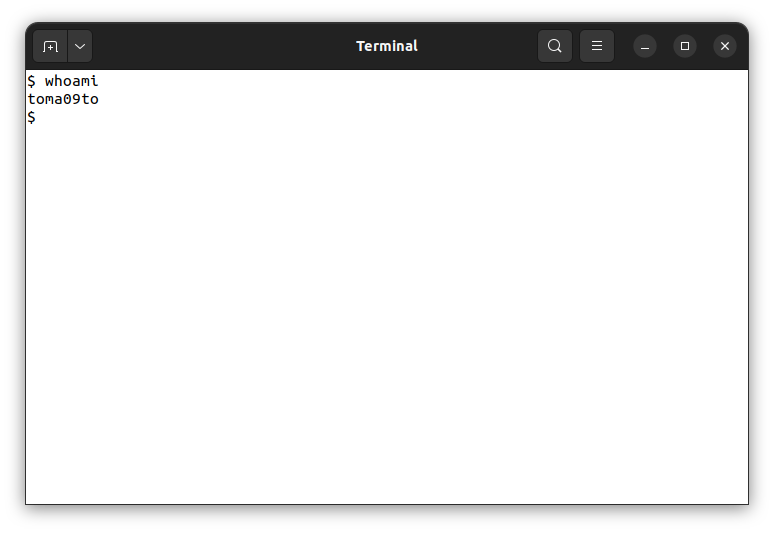
\includegraphics[width=100mm]{programming_template.png}
    \caption{図の例}
\end{figure}
\begin{table}[H]
    \centering
    \caption{データ型の最大値}
    \begin{tabular}{ c|c|c }
        データ型 & ビット幅 & 最大値 \\
        \hline
        char & 8 & 127 \\
        short & 16 & 32767 \\
        long & 32 & 2147483647 \\
    \end{tabular}
\end{table}

\section{数式}
プログラミングについて考えるとき、数式は欠かせません。
例えば、$l \times m$行列$A = (a_{ij})$と$m \times n$行列$B = (b_{ij})$の積$AB$を計算するとします。
この積を$C = (c_{ij})$とおくと、
\begin{equation}
    c_{ij} = \sum_{k=1}^n a_{ik}b_{kj}
\end{equation}
が成り立ちます。

これを各$i,j$について求めればいいので、プログラム(C言語)で書くと以下のような処理になります(ただし、C言語は0-indexedであることに注意)。
\begin{lstlisting}[language=myC]
for (int i = 0; i < l; i++) {
    for (int j = 0; j < n; j++) {
        c[i][j] = 0;
        for (int k = 0; k < m; k++) {
            c[i][j] += a[i][k] * b[k][j];
        }
    }
}
\end{lstlisting}
コードが3重ループになっていることから、この処理の時間計算量が$O(N^3)$であることが分かります。

\end{document}
